% !TeX root = ../report.tex

High Intensity Focused Ultrasound (HIFU) is a technique that uses non-ionizing ultrasonic waves to heat tissue in human body. It applies high-energy dose to the region of interest without harming the surrounding tissue\cite{JENNE2012311}. Due to the increase in temperature, it can lead to that the flow of blood or lymph is increased or unwanted tissue such as tumours are destroyed.  This technology is rapidly gaining popularity and is at various stages of development and commercialization.\cite{wp_HIFU}. For example, bone metastases causes chronic and severe pain to patients and hence lower their life quality significantly. HIFU can be used as thermal ablation technique in this situation and remove the tissue that causes the high pressure on nerves. Clinical trials have already shown promising results, where the patient's pain is immediately relieved\cite{vanwijk2013}. Other applications such as local release of medication encapsulated in temperature-sensitive liposomes are also gaining healthcare experts' interest.

When applying HIFU to patient, doctors want to monitor the temperature in affected tissues. Magnetic Resonance-guided High-Intensity Focused Ultrasound (MR-HIFU), as shown in Figure \ref{fig:HIFU_example}, is designed for this purpose. In an MR-HIFU treatment, the MR-thermometry is used to provide the temperature information for the doctors. However, this technique is limited when bone tissue is involved. Magnetic Resonance performs better in the rich-water tissues which have a long traversal relaxation time (T2)\cite{Modena_2018}. The distribution of water in bone is much lower than that of skin or muscle (22\% compared with 75\%). As a result, it has a shorter T2 and is harder to measure with high precision. What's making the problem even worse is that the temperature increase in bone tissue caused by ultrasound is faster than muscle tissue due to the different heat capacity.

\begin{figure}[h]
    \centering
    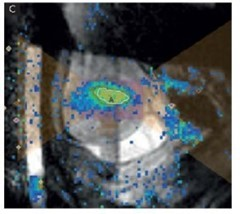
\includegraphics[width=0.5\textwidth]{HIFU-example}
    \caption{Real time temperature monitoring by MR-HIFU. The color indicates the chages in temperature. \cite{vanwijk2013}}
    \label{fig:HIFU_example}
\end{figure}

To solve this problem, computer simulation is introduced to help doctors estimate the temperature in bone tissue. Many methods have been developed to simulate HIFU system\cite{StochasticSim}. Most of them uses ray tracing method, which treats the ultrasonic wave as ray beam propagating towards acoustics medium. However, their performances are usually slow because they require the ray tracer to cast a great many rays so that the sampling of intensity can converge to realistic values. In this report, a new ray tracer is proposed which ultilizes the spreading of the beam to estimate the intensity, which can reduce the required ray casted and save some computational time.

The study can be divided into the following steps:

\begin{itemize}
    \item Implement Trident-Ray tracing method
    \item Set up experiment where there's only one medium.
    \item Set up experiment where there're two fluid media.
    \item Run the simulation on the second experiment with various different parameters.
    \item compare the simulation result with old simulation method on a similarity metric.
\end{itemize}
